\section{Introduction}
\subsection{What is HackerNews}
Hacker News is a social news site: it aggregates news by allowing users to submit stories. Interesting submissions can be upvoted by other users and all submissions are ranked by popularity.

The content on Hacker News is mostly related to science, in particular computer science. The guidelines for what content can be posted are very broad; the guidelines specify on topic as ``\textit{anything that gratifies one's intellectual curiosity}''\footnote{\url{https://news.ycombinator.com/newsguidelines.html}}.

Over the last eight years Hacker News has experienced rapid growth, resulting in a daily 2.6 million pageviews and 3.5 unique visitors per month\footnote{\url{https://news.ycombinator.com/item?id=9219581}}. One of the reasons suggested for this popularity is Hacker News' similarity to how Reddis used to be\footnote{\url{http://techcrunch.com/2013/05/18/the-evolution-of-hacker-news/}}: user-submitted content with a very minimalistic, terminal-like interface.

\subsection{Research Question}
The world changed a lot over the last eight years, especially in the field of computer science.  The userbase of Hacker News and their interests have changed as well. In this research, we want to see how they changed; what new . Informally phrased, we want to find trends in the popularity of several topics over the last eight years. This lead to the following research question:\\
\\
\textsc{Research Question:} how did the popularity of topics on Hacker News change over time?\\
\\
This question depends on two other questions, since we have not yet specified what we mean by popular nor what topics we mean exactly. These subquestions are:\\
\\
\textsc{SubQuestion 1:} how does one quantify the popularity of a topic?\\
\textsc{SubQuestion 2:} what topics does the Hacker News content consist of?\\

\subsection{Outline}
We will address the first subquestion by ranking posts and users over the entire Hacker News history. This will help characterize the dataset and show how various ways of measurent are often very similar and reveal some flaws in several ways of measuring popularity.

Dividing the content in topics is a more academically challenging task. We have used two methods to divide the articles into categories: latent Dirichlet allocation and a combination of Word2Vec and k-means. Both methods are briefly explained in section~\ref{sec:topic_detection}.

\section{Dataset}
As explained in the previous section, our analysis is on the set of all stories posted on Hacker News. It is a large set of news articles, blog posts, essays, tutorials and other types of textual media. Nearly all of it is English, although there are a few other languages used as well.

Let us first describe what exactly we refer to when we use the word story. To do this, we have to describe the various types of content on Hacker News, which can be catagorized in these four catagories:
\begin{itemize}
\item Stories: the majority of submissions are stories. A story can be either a link to another webpage or a relatively short text by the submittor.
\item Jobs: companies sponsored by YCombinator (the seed investor behind Hacker News) can post job offers on Hacker News. The percentage of Jobs is very small: well under one percent of the total volume.
\item Polls: users can submit multiple choice questions for other users to answer.
\item Comments: the three types mentioned above can receive comments by other users.
\end{itemize}

Since this research focuses only on the stories, we have left out the other three types. The dataset used in our research contains all stories between February 19th 2007 (the date Hacker News was launched\footnote{\url{https://news.ycombinator.com/hackernews.html}}) and June 10th 2015 (the day we ran our crawler). This is a time span of 3033 days, during which a total of over 1.5 million stories were submitted.

\textbf{+ 10GB comments for dictionary training data!}

\subsection{Data Retrieval}
To crawl all stories, we used the official Hacker News API\footnote{\url{https://hn.algolia.com/api}}. This API returns some basic data about the story, such as the submitter, title, points (upvotes), a (possibly empty) story text and a (possibly empty) url. Stories generally either have a story text or a url, most only have a url.

For the stories with a non-empty story text field, fetching the story from the API is enough. For other stories, we also fetched the content the URL links to. An important remark here is that some urls (especially the old ones) have become invalid over the course of time.

To crawl all stories (including the linked content), we used a homemade crawler that fetches the content, strips out meaningless text and html and saves the result in chunks of 1 day's worth of content. The code for this crawler is publicly available on GitHub\footnote{\url{https://github.com/bcleenders/AIM/tree/master/crawler}}.

The algorithm used for the extraction of meaningfull content is GoOse\footnote{\url{https://github.com/advancedlogic/GoOse}}. It uses heuristics to rank the importance and relevance of html elements on a webpage. For example: if it detects a \texttt{<div>...</div>} block with a lot of words inside, then that is likely to be important. If, on the other hand, it finds an html block \texttt{<button>Login</button>}, then it will remove the block for it is probably not a relevant part of the text of the page.

The resulting dataset is about 4.4 GB in size.

\section{Initial Analysis}
We have now established some semantics of the data gathered for our research. Before diving into the data analysis, we will first quantify the data by providing the reader with some statistics.

\subsection{Overall Activity}

\begin{center}
    \begin{tabular}{|p{3cm}|p{3cm}|}
        \hline
        \multicolumn{2}{|c|}{Statistics} \\
        \hline
         Stories & 1544261 \\ 
         Submitters & 165126 \\ 
         Upvotes & 16668848 \\ 
         Comments & 7383865 \\
         \hline
    \end{tabular}
\end{center}

An interesting remark, is that January 6th 2014 did not have any submissions. The reason for this was a long downtime of the Hacker News website
\footnote{\url{https://twitter.com/hackernewsonion/status/420068968464789505} - ``Hacker News is DOWN, but your chances of getting into YC if you know how to scale a plain text website are UP.''}.

\subsection{Upvote Distribution}
If users like a story, they can express their approval by upvoting it. These upvotes are then used to rank the stories by popularity and calculate the (currently) most popular submissions. Since the formula for determining a posts ``score'' strongly favours newly submitted stories, even stories with few upvotes can spike to the frontpage.

To enter the frontpage (the top 30), a story often needs at least ten upvotes, stories that stay on the frontpage for a longer period of time will often have over a hundred upvotes. The distribution of upvotes per story can be seen in figure~\ref{fig:distribution}. Stories placed in buckets of size 100 based on the number of upvotes they received. The graph plots the size of each bucket

Note that these graphs are scaled logarithmically: in the graph showing all posts (figure~\ref{fig:distribution_all}), 97.5\% of the stories are in the first bucket. That means only 2.5\% of the stories get over 100 upvotes. 

The second graph (\ref{fig:distribution_zoomed_in}) is a zoomed in version with a bucket size of 1, and shows the distribution for points with 30 upvotes or less, a set of over 1.4 million stories.

\begin{figure}[ht!]
\centering
\begin{subfigure}{.55\textwidth}
  \centering
  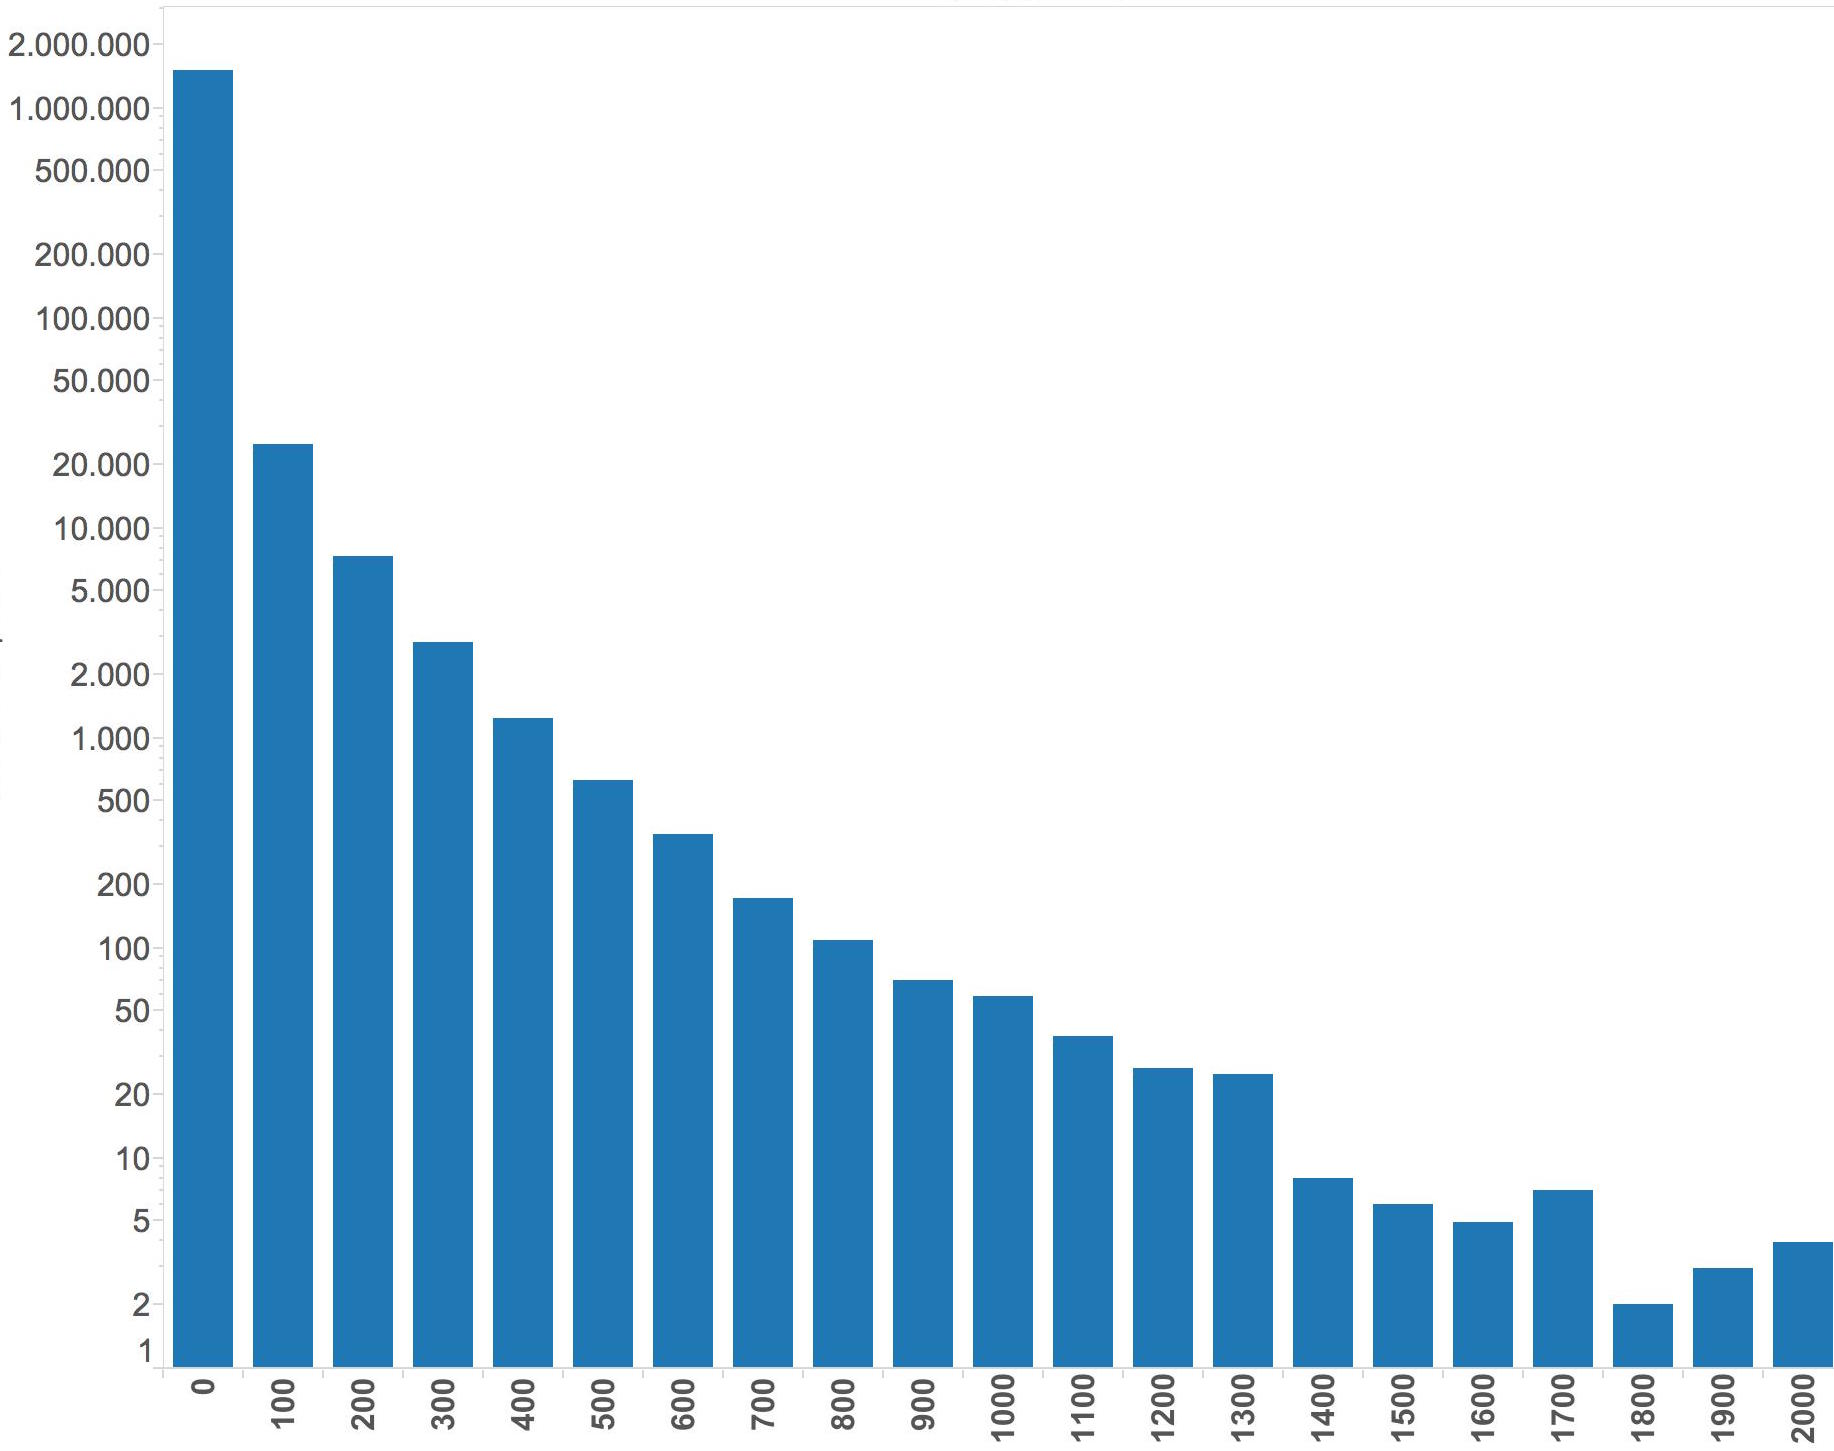
\includegraphics[height=6cm]{upvote_distribution_all}
  \caption{Distribution over all stories\\Bucket size 100}
  \label{fig:distribution_all}
\end{subfigure}%
\begin{subfigure}{.45\textwidth}
  \centering
  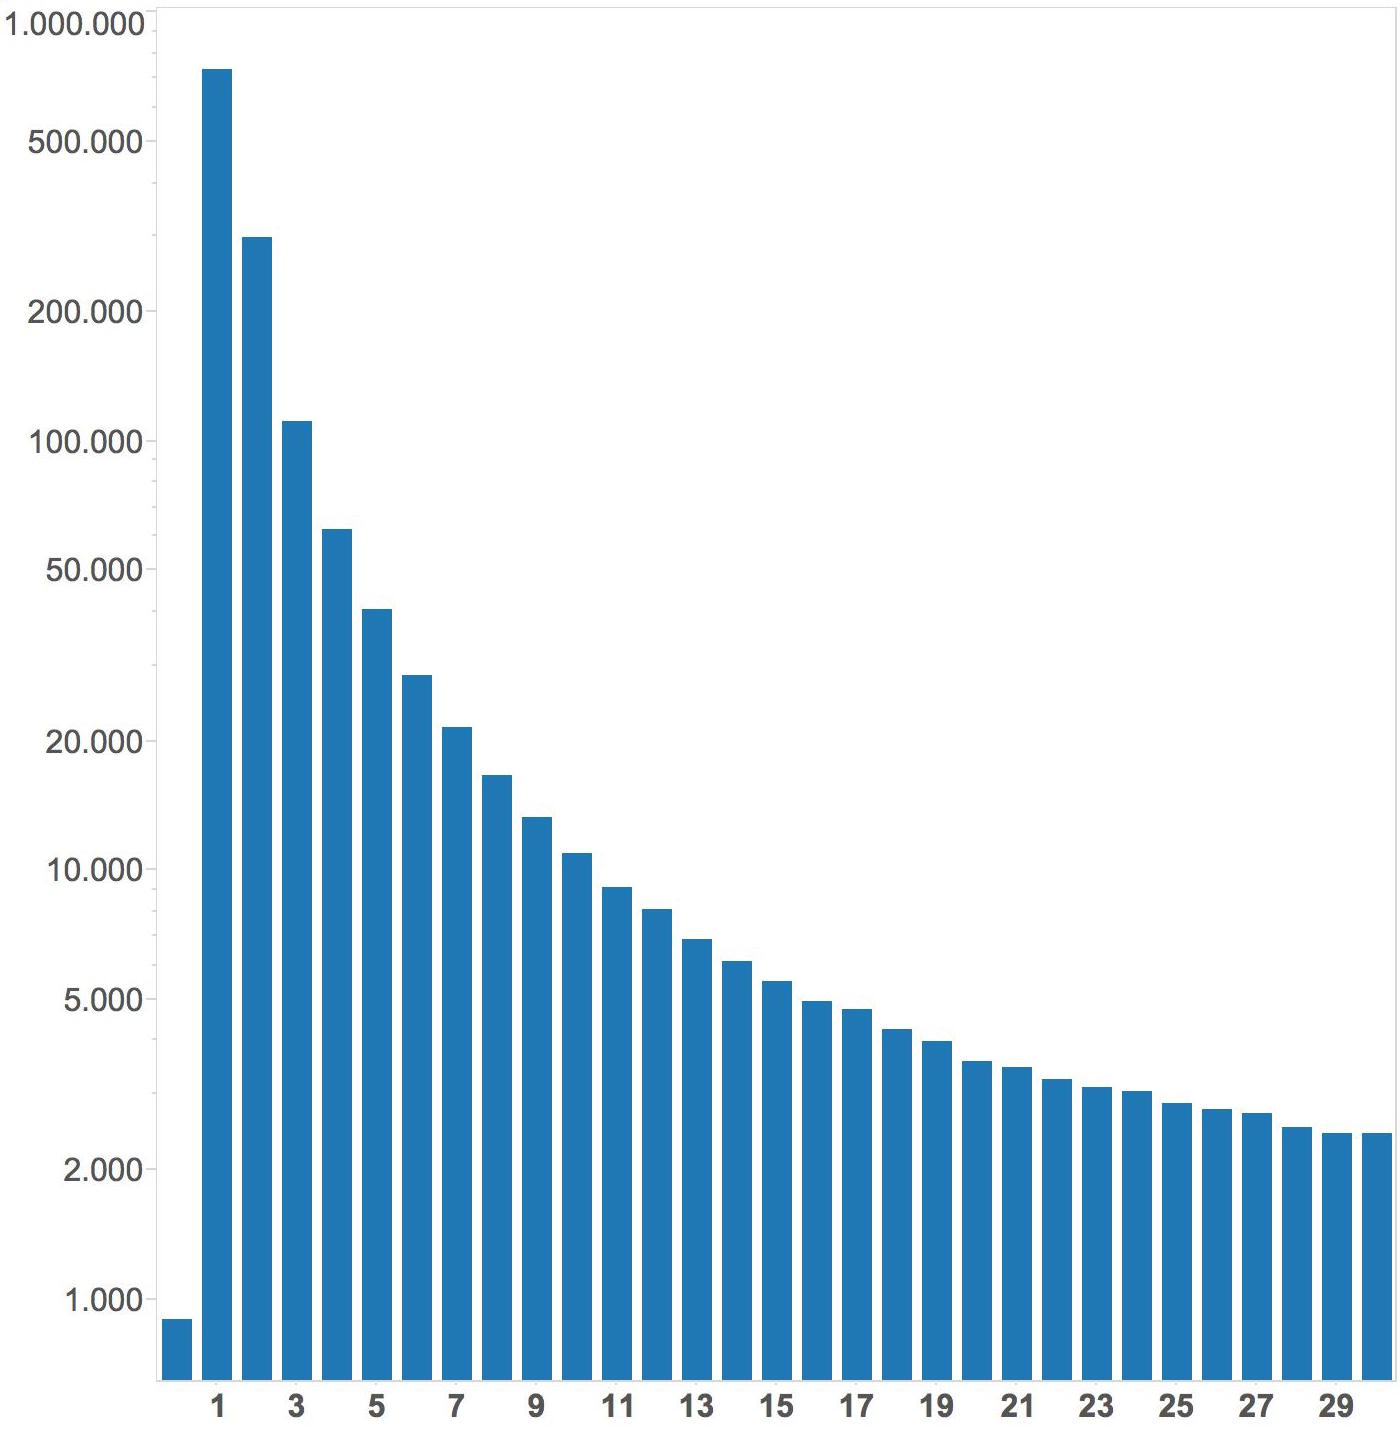
\includegraphics[height=6cm]{upvote_distribution_zoomed_in}
  \caption{Distribution over low-ranked stories\\Bucket size 1}
  \label{fig:distribution_zoomed_in}
\end{subfigure}
\caption{Distributions of upvotes over posts (log scale)}
\label{fig:distribution}
\end{figure}

There are only six stories with over 2100 upvotes. For completeness' sake, these are the stories whose popularity is quite literally ``off the charts'':
\begin{center}
    \begin{tabular}{|p{=8.5cm}|p{2cm}|}
       \hline
       \multicolumn{2}{|c|}{Most upvoted stories} \\
       \hline
       Title 																				& Points \\
       \hline
       Steve Jobs has passed away 										& 4271\\
		Tim Cook Speaks Up														& 3086\\
		2048																			& 2732\\
		Don't Fly During Ramadan											& 2617\\
		Hyperloop																		& 2549\\
		Microsoft takes NET open source and cross platform	& 2376\\
        \hline
    \end{tabular}
\end{center}

\subsection{Top Users}
In figure~\ref{fig:top10ByStories}, we show the statistics for some of the most active submitters. These statistics illustrate that Hacker News has a very active group of users. Together, this top 10 submitted 45,190 stories, which equals an average of 1.5 stories per user per day over the last 7 years.
\begin{figure}[ht!]
	\caption{Top 10 submitters by submitted stories}
	\label{fig:top10ByStories}
	\centering
	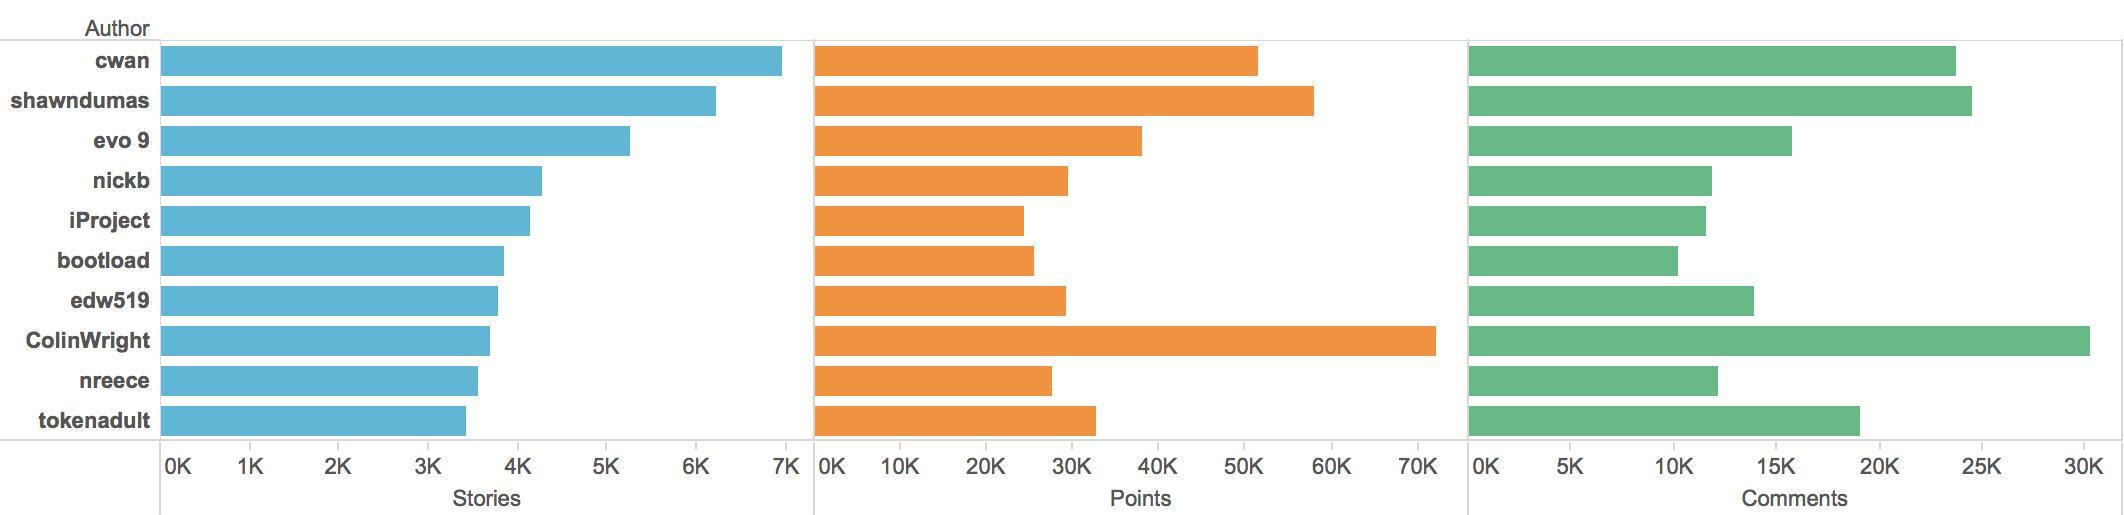
\includegraphics[width=14cm]{top10ByStories}
\end{figure}

If we take the top 10 not by the number of stories a user has submitted but by the number of comments his or her stories have received, we get the rankings in figure~\ref{fig:top10ByComments}.

\begin{figure}[ht!]
	\caption{Top 10 submitters by received comments}
	\label{fig:top10ByComments}
	\centering
	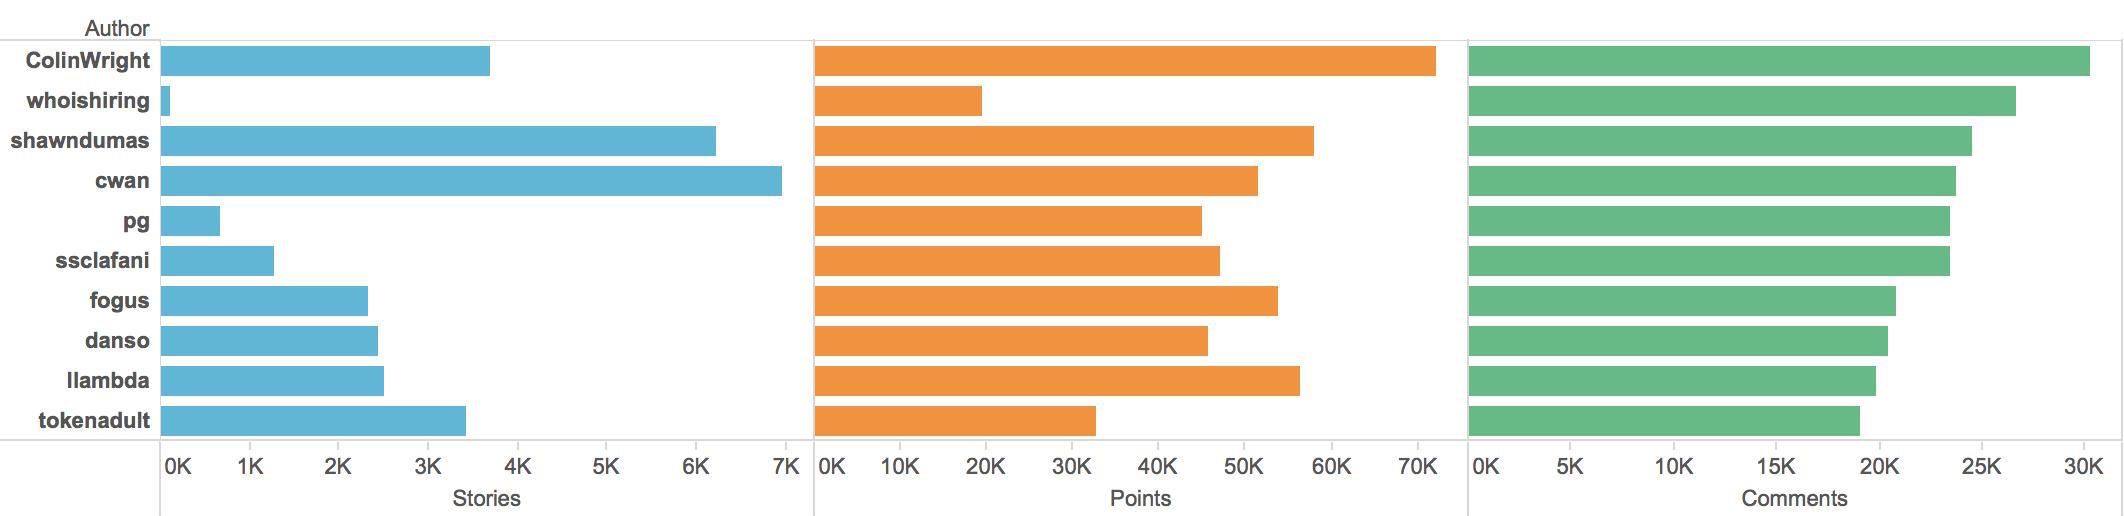
\includegraphics[width=14cm]{top10ByComments}
\end{figure}

The interesting second place in this top 10 is user ``\_whoishiring``. This user has almost no posts (a mere 114) but received 26,649 comments. Experienced Hacker News readers may have already expected this, for this user starts a monthly thread where companies can post job offers and others can respond to these. As such, the user only posts one story per month but its stories are discussed very actively.

\subsection{Top Domains}
As already stated in the description of the dataset, many of the stories are links to external sites. To provide some insights into which sites attract a lot of attention from the Hacker News community, we made three top ten lists that rank the sites by the same criteria as we did in the previous section: by number of stories, by points and by number of comments.

\begin{center}
    \begin{tabular}{|p{4.5cm}|p{=5cm}|p{5cm}|}
       \hline
       \multicolumn{3}{|c|}{Most popular domains} \\
       \hline
       By Number of Stories 			& By Points 									& By Comments \\
       \hline
       techcrunch.com (27.711) 	& github.com (400.373)		       & techcrunch.com (172.854) \\
		github.com (26.596) 			& techcrunch.com (365.207) 	   & nytimes.com (153.471) \\
		youtube.com (21.977) 		& nytimes.com (287.234)		   & github.com (127.812) \\
		nytimes.com (18.125) 		& arstechnica.com (176.633)	   & arstechnica.com (80.666) \\
		medium.com (14.172) 		& wired.com (161.698)		  	   & wired.com (75.406) \\
		arstechnica.com (12.657) 	& medium.com (132.468)		   & washingtonpost.com (56.257) \\
		wired.com (10.867) 			& bbc.co.uk (98.031)		  		   & medium.com (53.924) \\
		bbc.co.uk (8.118) 				& washingtonpost.com (97.537) & bbc.co.uk (51.828) \\
		en.wikipedia.org (7.058) 		& youtube.com (96.339)		  	   & theatlantic.com (41.530) \\
		businessinsider.com (6.877) & theatlantic.com (77.628)	   & online.wsj.com (36.729) \\
        \hline
    \end{tabular}
\end{center}

These rankings provide some insights into what types on news are popular. The big geeky news sites (Techcrunch, Ars Technica and Wired) are present and are about as popular as the big newspapers (NY Times, BBC, Washington Post). 

The high ranking of github.com (a code hosting site, \textit{not} a news site) can be explained by the large number of open source projects hosted on GitHub that submit links to new versions and press releases on Hacker News. Some examples of these projects are Facebook's React framework, Twitter's Bootstrap, SQLite and io.js. 

Notably, GitHub's competitors (e.g. BitBucket, GitLab and Beanstalk) do not show up in these rankings. This demonstrates GitHub's overpowering popularity in the code hosting market, at least in the open source community.

\section{Topic detection}
\label{sec:topic_detection}
It's data reduction and clustering, really...

Say that we did two types of unsupervised clustering: k-means and LDA. K-means

\subsection{Latent Dirichlet Allocation}
Some explanation what the F this is

\subsection{Word2Vec \& K-Means}
Explain two steps and how awesome it worked

\subsection{Discuss implementation}

\section{Results}
Make some awesome plots from the topics over time, rank by (upvotes | comments | number of articles published)

\begin{figure}[H]
	\caption{Topic group sizes}
	\label{fig:topicsizes}
	\centering
	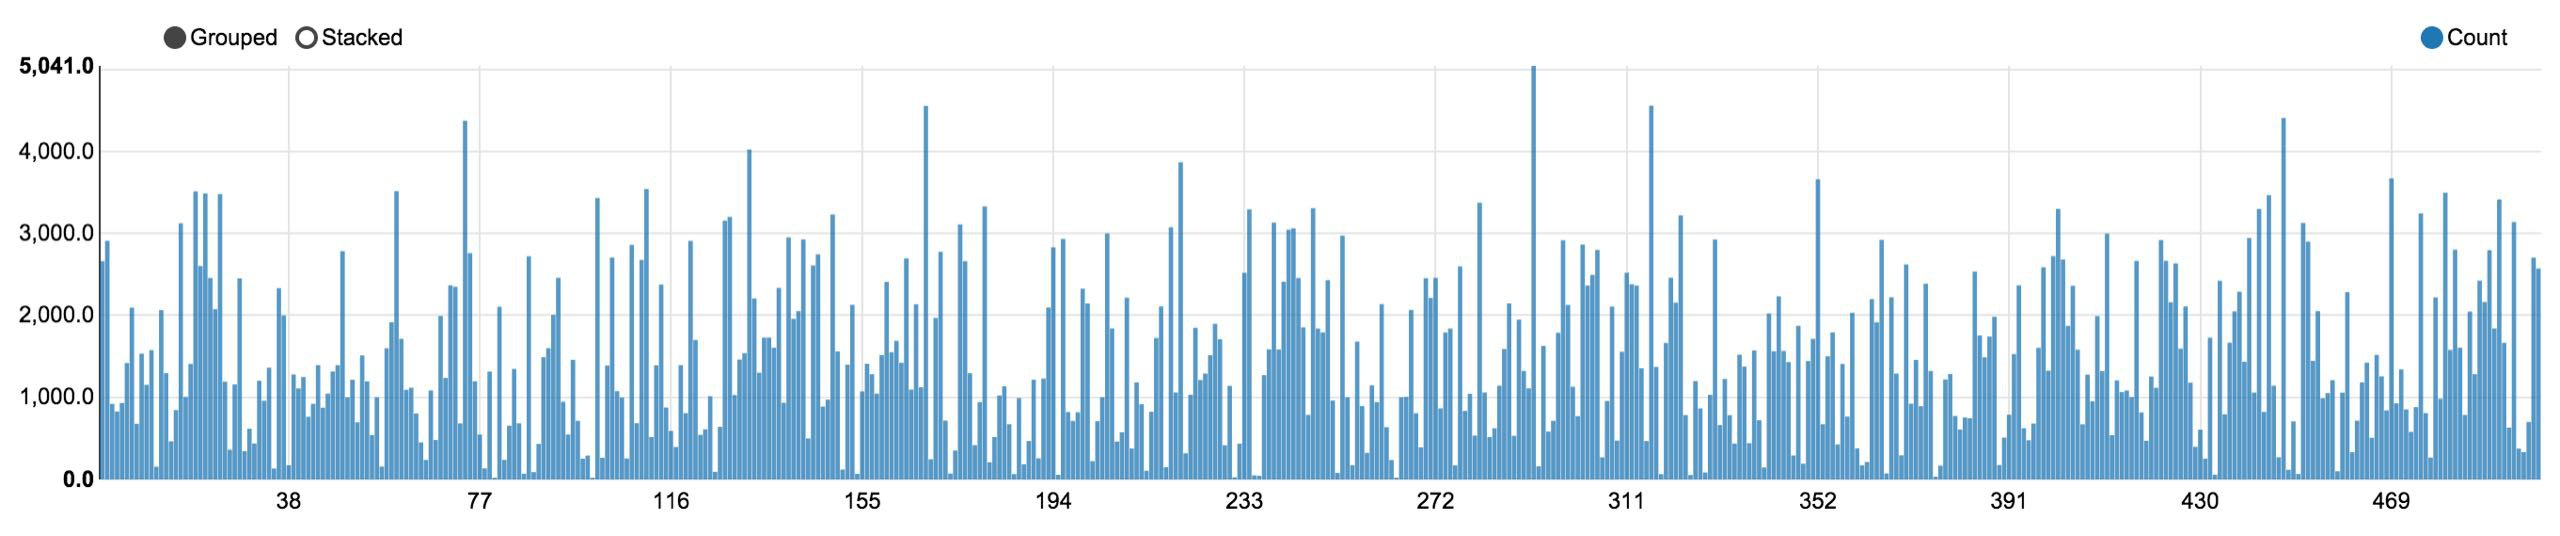
\includegraphics[width=14cm]{topicsizes}
\end{figure}

\subsection{Popularity plots}
In this section, we will show some awesome plots of how the popularity of various topics changed over time.

\begin{figure}[H]
	\caption{Popularity of Docker, CoreOS, etcd, containers, OpenStack}
	\label{fig:trend_docker}
	\centering
	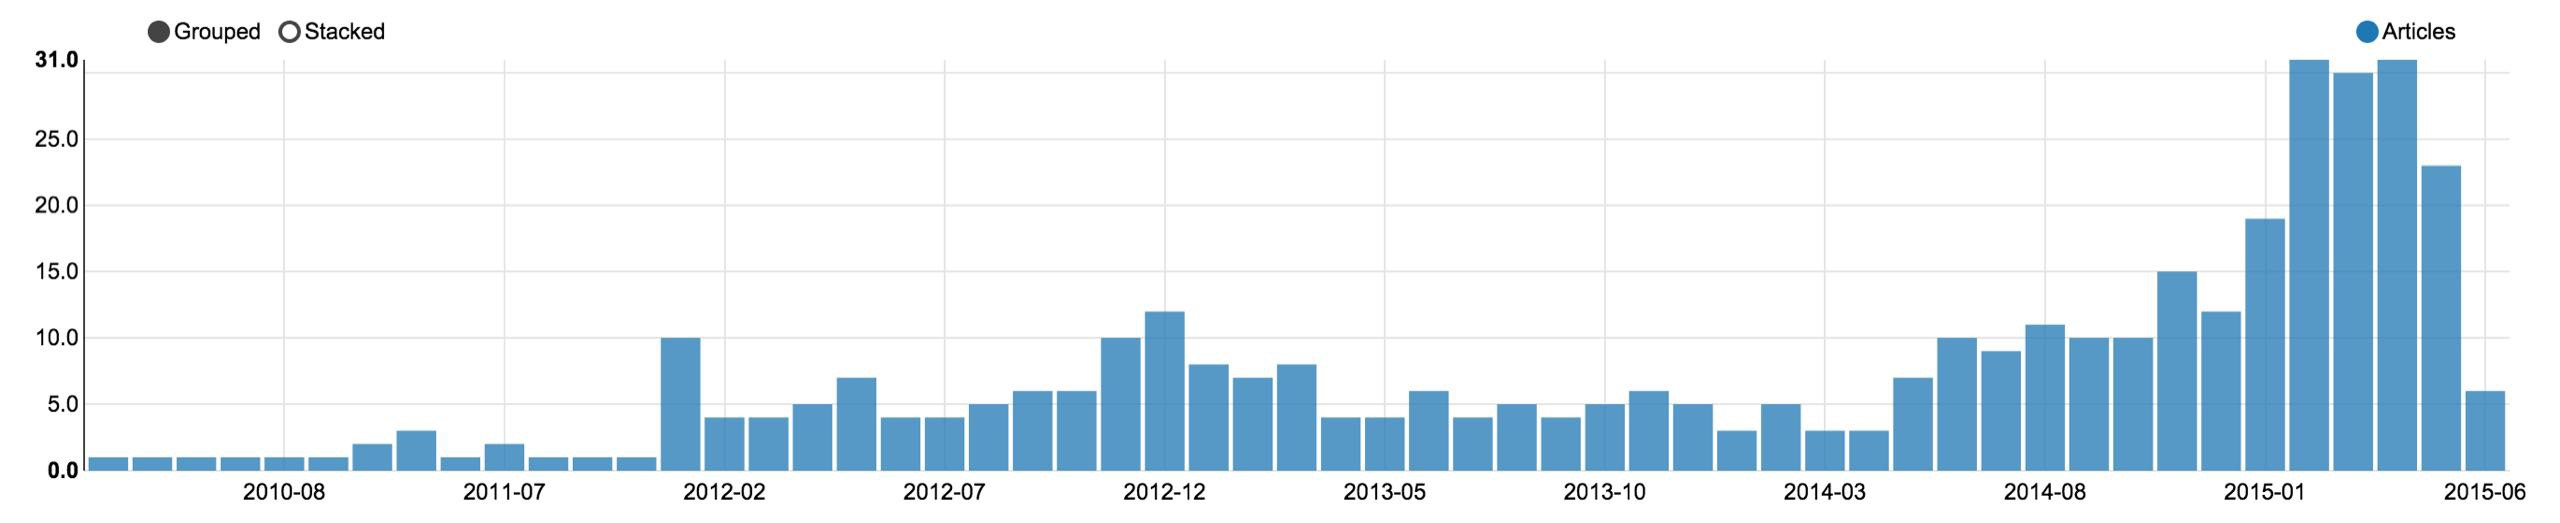
\includegraphics[width=14cm]{topic_trends/docker}
	% docker coreos etcd images:containers openshift mesos deis openstack orchestration dokku
\end{figure}
We start the overview with a trend plot (figure~\ref{fig:trend_docker}) of a new and upcoming technique: containerization. Docker and CoreOS were released in March resp. October 2014 and before that, containerization was already used as a term for seperating Linux processes. The trends show how Docker started gaining some real traction within half a year and is really booming in the first half of 2015.

\begin{figure}[H]
	\caption{Popularity of Elon Musk, SpaceX, Tesla, Hyperloop}
	\label{fig:trend_elon}
	\centering
	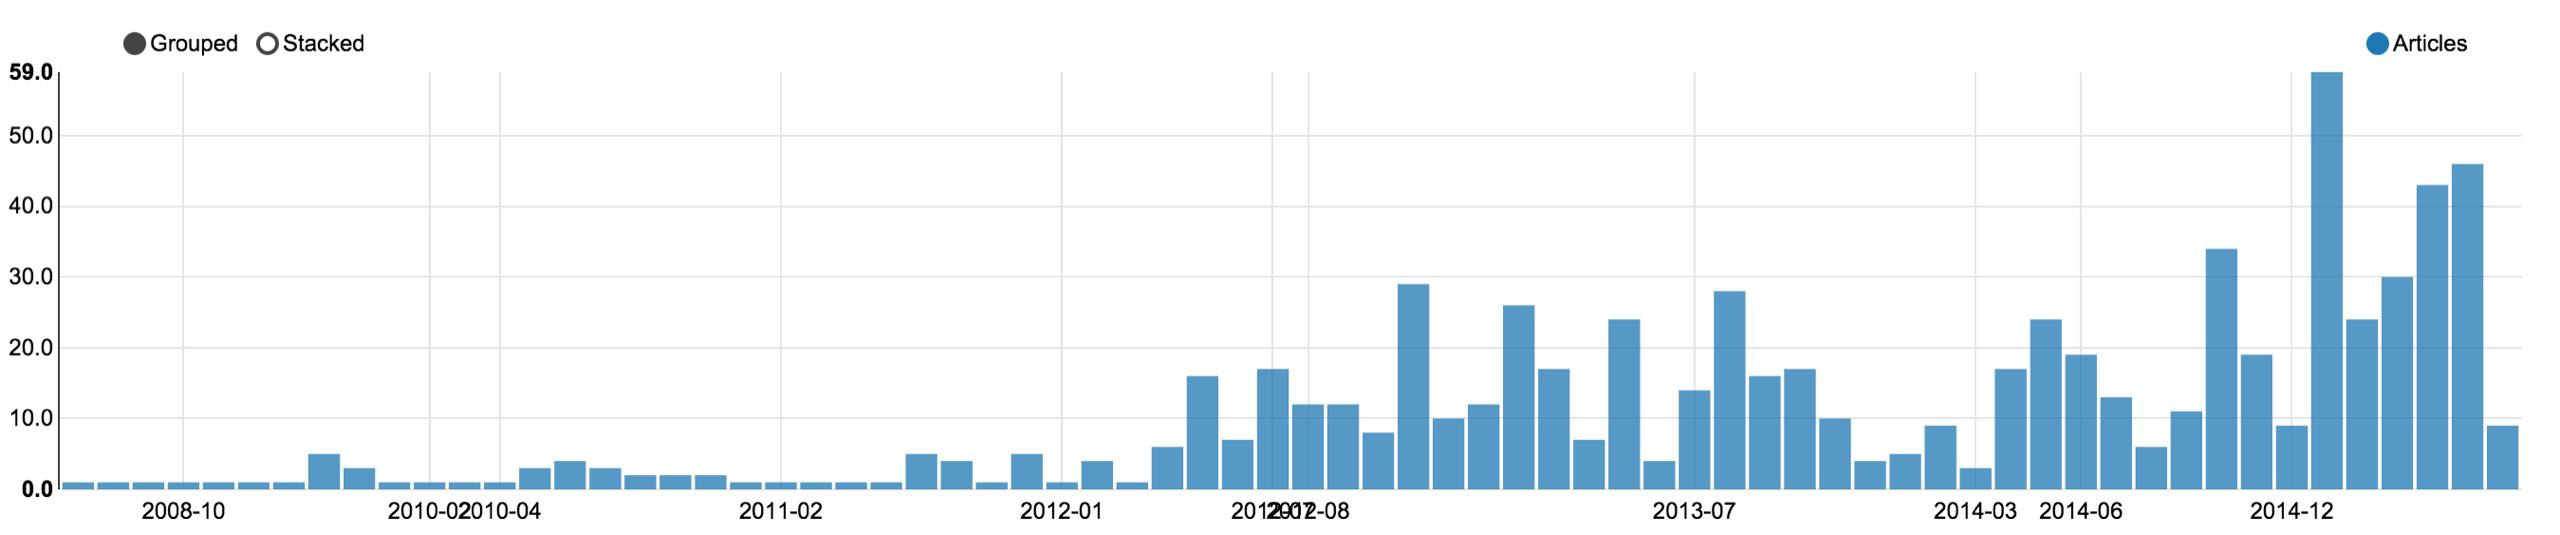
\includegraphics[width=14cm]{topic_trends/elon}
	% elon musks spacex musk's tesla hyperloop test track musk
\end{figure}
\textbf{Something about Elon's awesome projects :)}

\begin{figure}[H]
	\caption{Popularity of keynote, Apple, live, @scale, conference}
	\label{fig:trend_keynote}
	\centering
	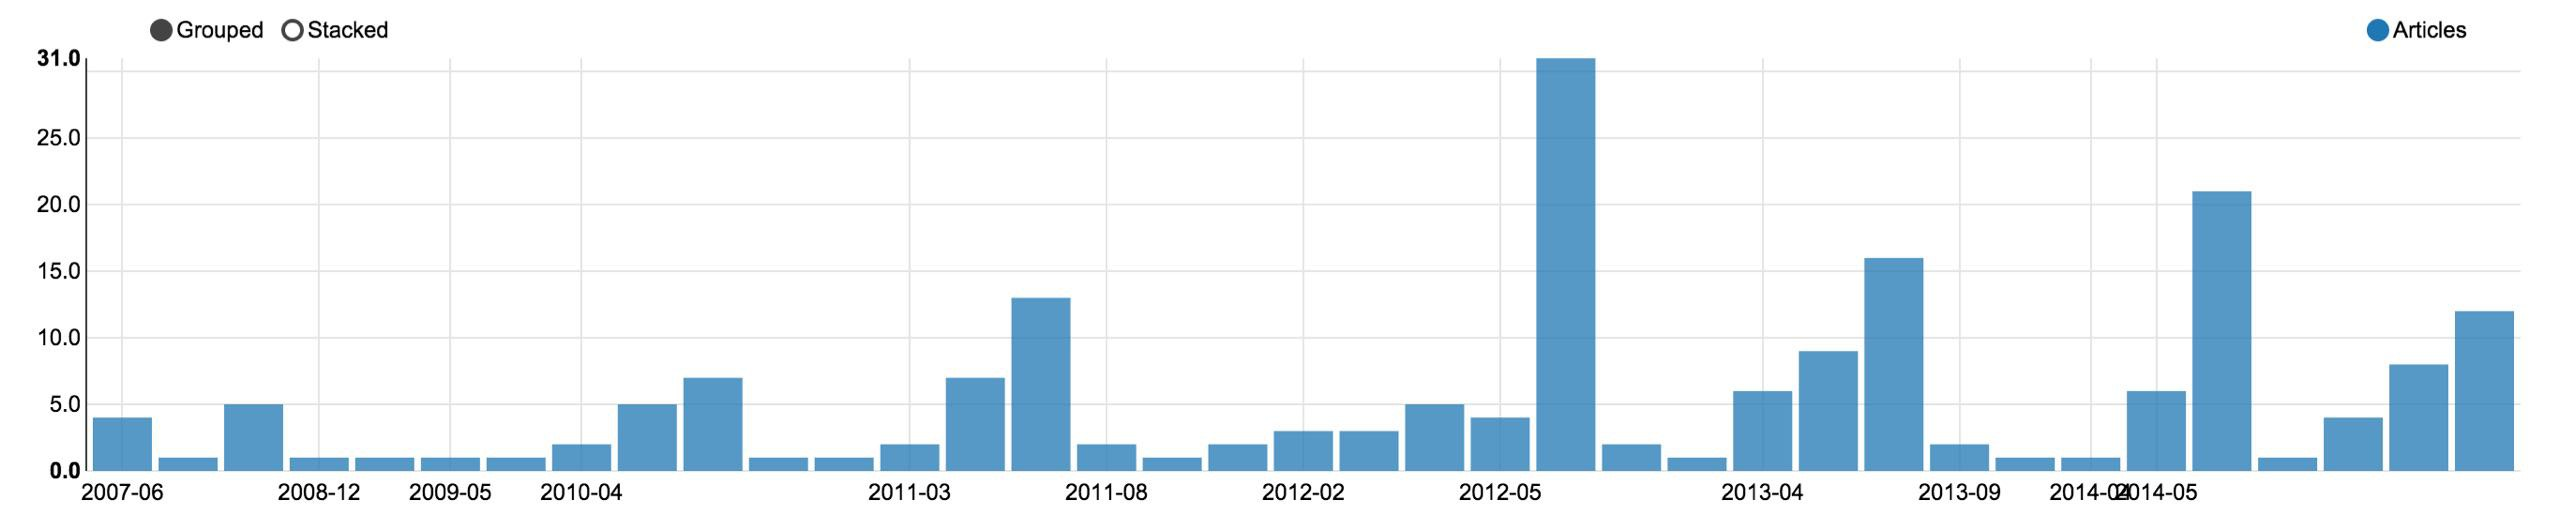
\includegraphics[width=14cm]{topic_trends/keynote}
	% keynote apple live yesterday's apple's @scale apple developers conference keynotes conference macworld
\end{figure}
In the popularity charts of keynote-related topics (figure~\ref{fig:trend_keynote}), one can see patterns of three months of increasing popularity. The highest point is always the month in which an Apple keynote took place; the two months before usually have rumours about what new products will be introduced.

The big spike halfway 2012 marks the announcement of Siri, Apple's articifial intelligence personal assistant.

Unfortunately, Hacker News started after the release of the iPhone (January 2007; one month too early), so we cannot see the data for that release.

\begin{figure}[H]
	\caption{Popularity of Steve Jobs, Wozniak, imagineers}
	\label{fig:trend_jobs}
	\centering
	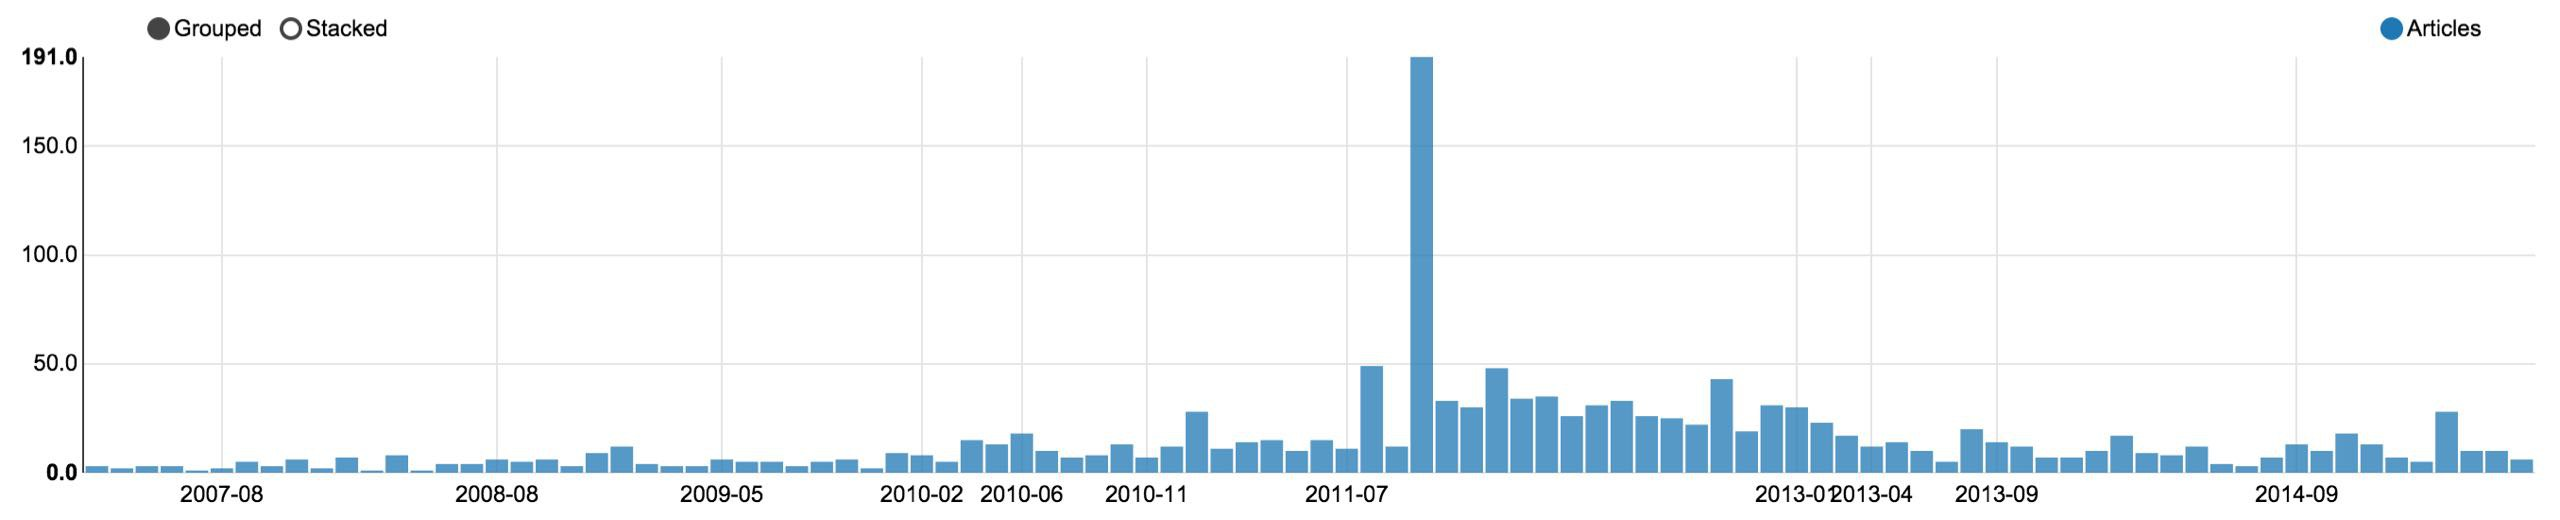
\includegraphics[width=14cm]{topic_trends/jobs}
	% jobs wozniak woz jobs. steve steves jobs's jobssteve imagineers wozs
	% Interesting: Tim Cook is not in this cluster, and his coming out is therefore not visible in this graph
\end{figure}

On the topic of Apple: not only it's products spark the interest of the Hacker News community; it's former CEO also had a big impact in the community. We show figure~\ref{topic_trends/jobs} to indicate the enormous impact the death of Steve Jobs had. He shares this topic group with his co-founder Steve Wozniak, but the news of his death (October 5th, 2011) dwarfs all other events in Hacker News history.

\begin{figure}[H]
	\caption{Popularity of Raspberry Pi, Kindleberry}
	\label{fig:trend_raspberry}
	\centering
	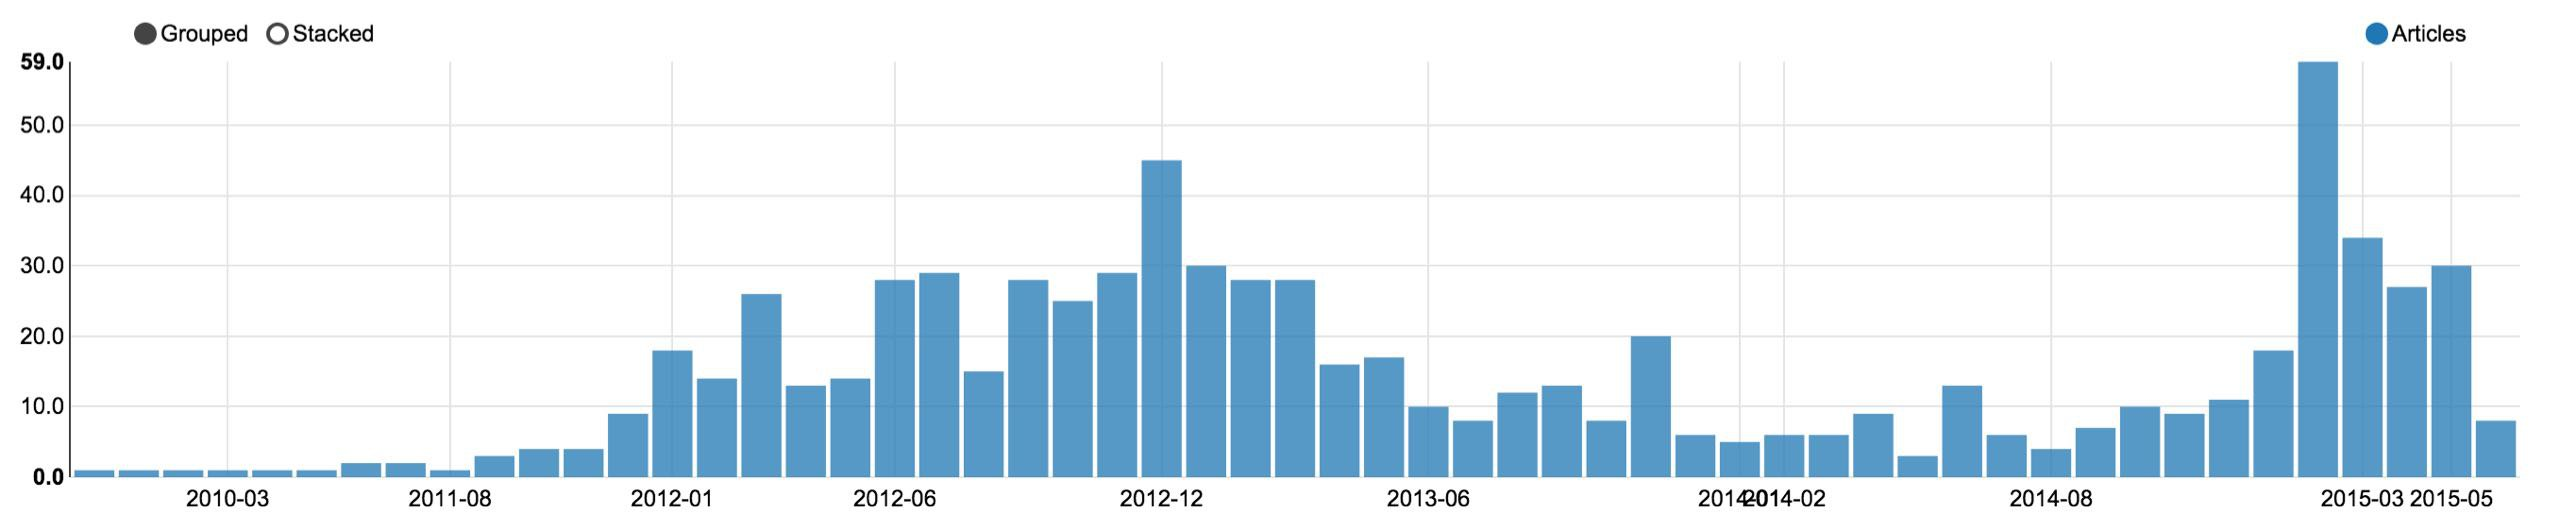
\includegraphics[width=14cm]{topic_trends/raspberry}
	% raspberry pi's kindleberry pis navio+ motherbone-tm-pione-tm- piface razberry rpi raspberrypi
\end{figure}

\begin{figure}[H]
	\caption{Popularity of Edward Snowden, Wistleblower, leaks, Reddit}
	\label{fig:trend_snowden}
	\centering
	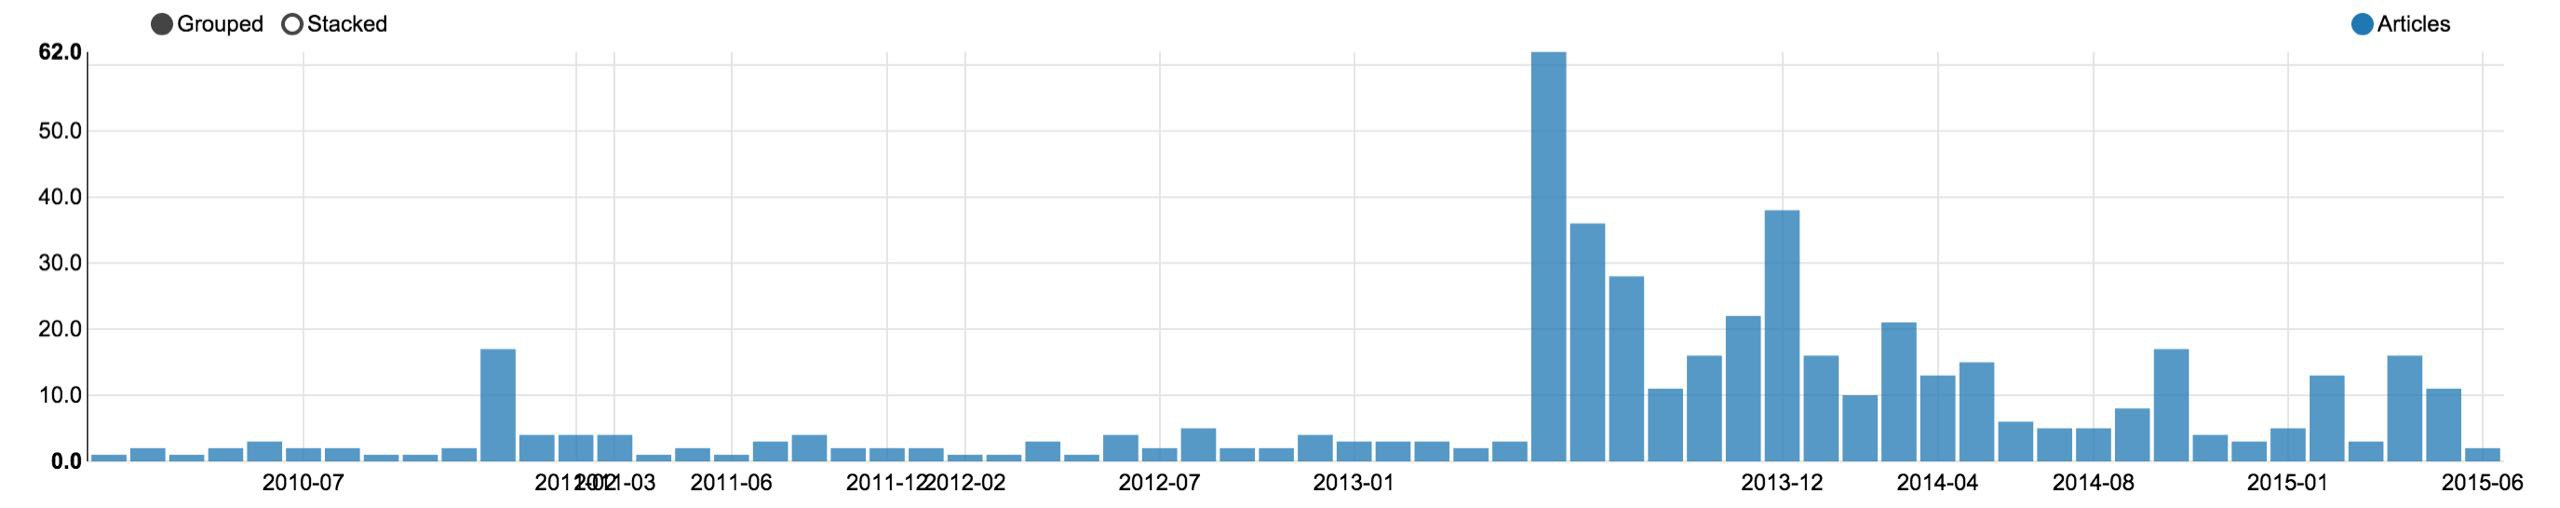
\includegraphics[width=14cm]{topic_trends/snowden}
	% edward whistleblower contractor-turned-whistleblower snowden.the snowden's leaker snowdens reddit.comsubmitted snowden. snowden.in
\end{figure}



\section{Conclusion}
We`re awesome!